\section{Simulation} \label{sec: Simulation}
%Describes the result of the behavioral simulation based on the synthesized hardware description language.
%The most important module to simulate is the state machine because it includes the logic applied out of the state diagram. 
%One problem by simulating out of the top level are the clock divider which would need way more simulation time then 1000 ns therefore it is good practice to simulate each module once and proof its function by writing individual test bench files for each module.
%Figure \ref{fig: Simulation_state_machine} shows the simulated state machine with the state gum. By using radix for the char01 to char 12 signals an easy readable simulated result can be achieved.
%For an extended report more simulations would be added and explained in more detail.
%
%\begin{figure}[H]
%	\centering
%	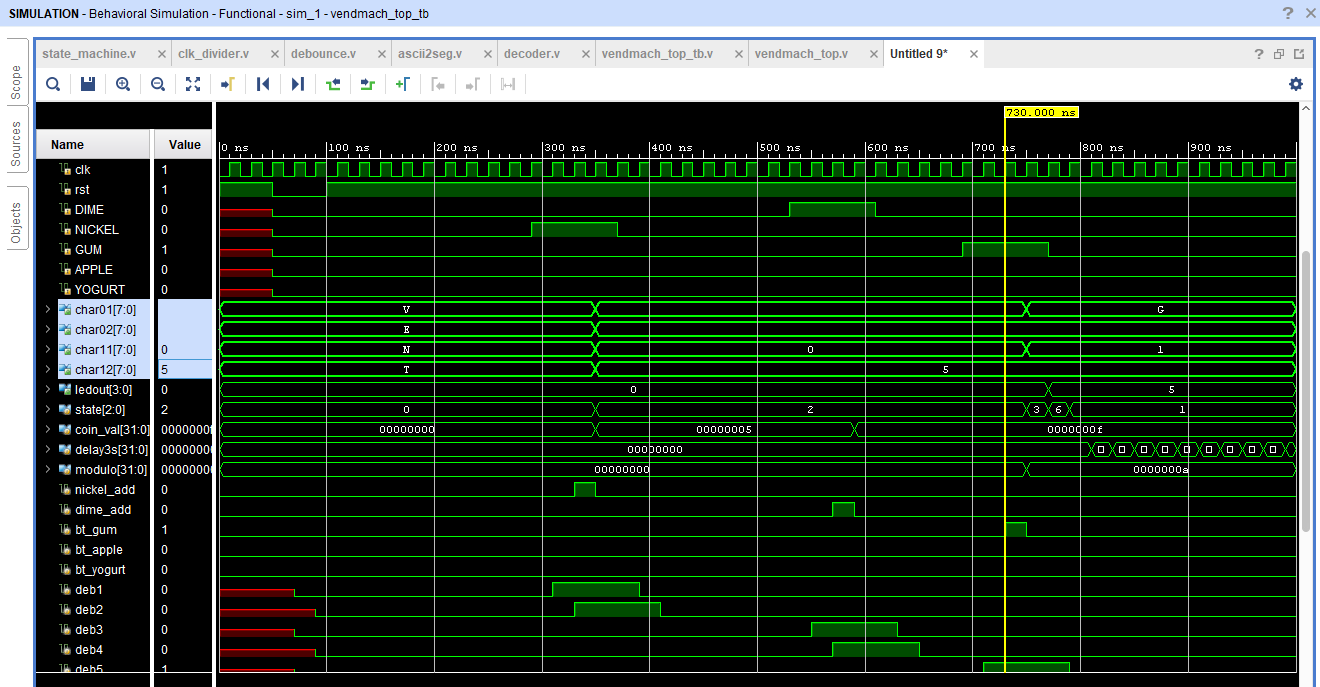
\includegraphics[width=1.0\textwidth ]{01_images/Simulation_state_machine.PNG}
%	\caption{Vivado behavioral simulation of the state machine module.}
%	\label{fig: Simulation_state_machine}
%\end{figure}

